\chapter{STOCKS AND BONDS}
\begin{chapquote}{Ariel Deschapell}
``While traders may move the markets, it is the tinkerers that will truly determine the future.''
\end{chapquote}

\section{Introduction to stocks} \label{Introduction to stocks}

If you own shares, also known as stocks, you are a part owner of a company. If you own bonds, you are part lender to the company. A company, just like a normal person, has assets, say $A$, and liabilities, say $L$, with a resulting equity $E = A - L$. Let's assume also that the company decides to have $N$ shares. This means that the value of each share is $V = \dfrac{E}{N}$. So, if you own $n$ shares of this company, you'd have a total amount of $S = V \cdot n$. Now, $A$ and $L$ are values provided by the company itself, but the market may perceive the value of the company in a different way. This means that people may be willing to sell and buy shares for a price different from $V$, say $V'$. If the company is known to have a good outlook, then $V' > V$. The market capitalization is simply $C = N \cdot V'$, which can obviously be different from the equity $E$.

There are two ways for a company to raise money: by borrowing money (debt) or by selling shares (equity). A security\footnote{A security is something that can be bought and sold that has some economic value. Possible categories are: debt securities (e.g., banknotes, bonds), equity securities (e.g., common stocks), derivatives (e.g., forwards, futures, options, and swaps).} in the former case is a bond, while in the latter is a stock. As we can split the equity in shares, we can split liabilities in bonds\footnote{Of course, we can have part of liabilities in form of loans with banks instead of bonds with the market.}, meaning that our debt can be owned by someone with these bond tickets. This ticket says the company will pay back the money to its owner at maturity. A stock is different in that its ownership does not mean the company owe me money.

\section{Shorting stocks}

Let's say I have reason to believe that the stocks of company X are going to lose value in the near future. The current share value is $V$. What I do is going to a broker and ask him to borrow\footnote{When borrowing stocks, in general there is a upfront payment of 50\% of the stock value.} me some stocks, say $n$ from company X. Let's assume the broker has $N$ stocks from company X owned by some of his other clients and he's able to lend me $n$ stocks\footnote{Once I have the shares, it is still as if the original clients own the stocks, so if there are dividends from the company I have to pay for them to the original owner of the stocks and the broker has to make sure that everything plays out smoothly. The original owner of the stocks is aware of her stocks being borrowed to me, but she can still sell them. To do this, the broker will give her stocks from another of his clients and then it's as if I borrowed the stocks from this second client.}, where $n < N$. Then, what I do is to sell these $n$ stocks to the market and I get a revenue of $R = n \cdot V$, but I still owe $n$ stocks of X to my broker. Luckily, after some days the value of the stock decreases by 50\% and I decide to cover and buy $n$ stocks from the market spending $C = n\dfrac{V}{2}$ and I give them back to my broker. At the end, my profit is $P = R -C$. In this case I'm the short seller: I borrow and sell high (shorting) and I buy low (covering), while long sellers are people who buy low and sell high. A regular trader would make money by buying low and selling high and buying low and selling high and so on. Depending on where you start from, you are a good long-seller or a good sort-seller.

In this case, the short seller (me) was lucky because the company's shares did lose value. What if the shares went up instead? Imagine that, as time goes by, the share's value keeps increasing. The more I wait to cover my stocks (buying them from the market and giving them back to my broker) the more the money I lose. In this short-selling scenario, there is absolutely no limit to the money I can lose. If the company keeps reporting good results for years, I may end up with a huge amount of money to pay back to my broker. In the case of long selling instead the worst case scenario is me losing the initial amount of money I used to buy stocks, which is limited, whatever the losses of the company. 

In a financial market with only good short-sellers, the volatility of the market would be reduced. Why? A successful short-seller would sell when the stock value is high, and if there are lots of successful short sellers the value of the stock would decrease, (simply because there is more stock supply). When the stock value is low instead there are a lot of buyers and the stock value would increase (simply because there is more demand). Bad short-sellers would make the stock more volatile instead, but they will disappear soon from the market as they'll lose lots of money for being bad short-sellers (buying high and selling low). In general, the owners of a stock don't like volatility.

The are two types of people in the financial market: the ones who are positive and the ones who scrutinize. The first group wants markets always to go up. They report good news, try to hide problems to avoid losses. Some examples are companies' management, banks, governments, ads sellers (mostly financial press), rating agencies (paid by banks). The second group is basically made of short-sellers, who try to find problems in companies, banks and governments. They try to make sure that the value of stocks, and in general the markets, are not overvalued. They can be seen as being in the society's side in preventing bad behaviours from the positive group. Of course, there may be some exceptions such as people spreading rumours and manipulating the markets.

\section{Understanding company statements and capital structure}

As seen in section \ref{Introduction to stocks} the market capitalization $C$ can differ from the owner's equity $E$ if the market as a different view compared to the company's books. If the market capitalization is higher than equity, it means that the company has an intangible asset, which could be the brand itself, the management's expertise or the location for example. What if the market cap is lower than equity? It means that the assets of the company do not actually worth that much.

\section{Corporate metrics and valuation} \label{Corporate metrics and valuation}

By selling a product, a company gets revenues, from which it subtracts the cost of the products, resulting in the gross profit. Then it subtracts other additional costs generally known as Selling, General and Administrative Expenses (S\&GA)\footnote{Direct labor is employees who are directly involved in making the product, who "touch the product." The labor cost is included in cost of goods sold. Everyone else is considered indirect labor and included in SG\&A.} to obtain the operating profit $P_{op}$. The return on asset is then computed as $ROA = P_{op}/A$, where $A$ is clearly the assets of the company. If the company owns some stocks or other financial assets, then the real return on asset is $ROA = \dfrac{EBIT}{A}$, where the numerator stands for earnings before interests and taxes which is equal to the operating profit (profit coming from the operating assets) plus the profit from financial assets that the company owns. This second definition is a bit more informative than the previous one. In general the return on asset tells us how good a company is in turning its assets into money, ignoring loans and taxes.

Some companies though may have some liabilities, such as loans to banks, so they need to subtract the interest to pay from the operating profit obtaining the pre-tax profit\footnote{Most companies pay the interest on the debt rather than paying the principal of the debt because they will have higher deductible taxes.}. As expected, from the pre-tax profit one must subtract taxes to get the net income $I_{net}$, also known as earnings, usually reported a TTM (trailing twelve months). Another index for evaluating a company is the return on equity $ROE = \dfrac{I_{net}}{E}$. This indicator could also be seen as how good the company is at dealing with loans and taxes.

If a company has $N$ shares, then the earning per share is $EPS = \dfrac{I_{net}}{N}$. Instead, the price to earning ratio is $P/E = \dfrac{V'}{EPS} = \dfrac{NV'}{I_{net}}$, where $V'$ is the value of a share determined by the market, which can, as already said, differ from the book value per share $V$, determined by the accountants of the company. What's the meaning of this $P/E$\footnote{Be careful: the denominator stands for earnings and not equity.}? It represents how much money you have to invest on a single stock to get a profit of one dollar (or any other currency). Obviously, the lower the better because a small numerator and a big denominator means I pay few for something that will give me more. If you look at it from another perspective, namely its inverse, $E/P$, it can be seen as the percentage of profit you make with an investment. If an earning per share $EPS$ is always constant and the price to earning ratio $P/E$ is low (or equivalently a high $E/P$), you should invest on that company rather than putting your money into the banks which usually offer a lower interest rate compared to the $E/P$ of the company―because banks bring less risk in general\footnote{Usually banks offer few percent points in interest rates, say 2\% which means a $P/E$ of 50.}. Usually, companies are analyzed in depth to assess their future earnings or equivalently their future $EPS$, and the final result of all the analysts is averaged and a consensus is expressed in the so-called forward earnings. These are sell-side analysts from investment banks and research houses that are trying to sell financial products. In contrast we have buy-side analysts, namely people from hedge funds that must decide where to invest.

If two companies have two different $P/E$ ratios, it is not always better to buy the one with the lower value. Why? First of all, the one with lower value may be more risky. Second, the one with higher value might be growing and its $P/E$ will decrease. You can also see it in this way: if a lot of people are willing to pay a high price for a stock, it means the company is believed to grow, if instead the price is low, maybe the stock is not very interesting for the market. A low PER can indicate either that a company may currently be undervalued (people do not believe in the company despite its profit) or that the company is doing exceptionally well relative to its past trends.

An individual company’s P/E ratio is much more meaningful when taken alongside P/E ratios of other companies within the same sector. For example, an energy company may have a high P/E ratio, but this may reflect a trend within the sector rather than one merely within the individual company. An individual company’s high P/E ratio, for example, would be less cause for concern when the entire sector has high P/E ratios.

The price to earning ratio is useful to represent the growth of a company, but it does not consider how the company is capitalized, namely how the assets are payed. The enterprise value is obtained by adding the market cap to the debt and subtracting the non operating assets (cash, financial investments): 
\begin{equation}\label{ev}
    EV = C + L - A_{non-op}.
\end{equation}
To obtain a more correct share value, an investor chooses a price to earning ratio for the company that he's willing to pay and sets it equal to the ratio between the enterprise value and the operating profit:

\begin{equation}\label{eq:pe_ev}
P/E = \dfrac{EV}{P_{op}}.
\end{equation}

From equation \ref{eq:pe_ev}, we can obtain $EV$, which then can be used in equation \ref{ev} to compute the market cap $C$. The price per share the investor is then willing to pay would be $PPS = \dfrac{C}{N}$, where $N$ is the number of shares. In this way, if two companies have the same operating profit but different liabilities and non-operating assets you'd buy stocks from those 2 companies at different prices.

Another index to analyze a company is the ratio between enterprise value and EBITDA (earnings before interests, taxation, depreciation and amortization). The difference with ROA―where the denominator was operating profit―is that here we don't consider depreciation and amortization which are non-cash expenses, rather we consider raw cash that the company is producing. EBITDA represents how much income the employees are generating by their current activities. It ignores things that employees have nothing to do with.

\section{Life of a company} \label{Life of a company}

It all starts with an idea and some unique skills. These are the only (intangible) assets of the company. The founders can issue shares to themselves and decide what is the value of their idea before starting the business. Let's assume they agree on a sum $S$, which is the pre-money valuation. What they need to do then is to find an investor. Banks are not helpful in this case, but venture capitalists or angel investors might be interested in the idea and put a sum $S'$ to start the business. This sum may be higher than the pre-money valuation and if this is the case, the investor will own the majority of the shares. Now the assets are both intangible (the idea and the skills) and tangible (the investor's money) for a total of $S + S'$, the post-money valuation. This means that the owners must issue shares for a total amount of $S'$ to the investor. 

Once the business has started―an office, employees, and so on―the founders might need additional money to go on because they didn't make much profit yet. In this case, the founders ask for help to seed venture capitalists, more professional people. The money from this seed VC investor represents the series A founding. The seed VC has MBAs and analysts for a pre-money valuation, say $S''$ which can be more, but also less than our previous assets $S + S'$, which means our shares will be worth more or less. The founders and the other owners may decide to get the series A funds also at a lower value so as not to lose the majority in the company. The post-money valuation of the company will be then $A =S + S' + S''$, assuming $S''$ is the definitive series A funding, and the owners will issue more shares to the seed VC according the new funding value. If more money is needed, the owners will raise a series B funding with other VCs and issue more shares. Up-round is when the pre-money valuation of this round is higher than the post-money valuation of the previous round. 

The problem so far is that the investors own shares of the company, but they cannot turn them into cash. The board can then decide to go public and raise a lot of money with an initial public offering (IPO). The legal work will be carried out by the legal underwriter and a syndicate (group of investment banks) will come up with a price. This price should allow the stock value to increase in the first days, so it shouldn't be too high. If the stocks are bought during an IPO, this money will finance the company, but if the stocks are traded afterwards in a stock exchange, no additional money will be received by the public company. Usually a 7\% of the money raised is payed to the syndicate. After some time, if the company needs more money, it can issue more stocks and sell them to the public market (probably a lower price as the offer increases). This is called follow-on offering.

When a company is going bad, it has two options: liquidation (called chapter 7) and restructuring. Liquidation means that the assets are sold to pay back the debt in the liabilities and then the company shuts down. The debt is layered: senior secure, senior unsecure, subordinated, junior (equity). The first level is the one which is paid first. The other option is when the shareholders think the company can still operate but the debt is too high. What happens is that the company starts chapter 11 bankruptcy and gets a new loan: Debtor In Possession Financing, which is even more senior than the senior secure, to keep operating. Then, the bankruptcy court (group of banks) will value the company (its assets) and how much debt it can have, someone will provide higher numbers (people related to the shareholders) and someone else will provide lower numbers (banks hired from the seniors). The lower the valuation, the higher the number of the shares the seniors will get, vice versa the higher the valuation, the higher the numbers of shares the original shareholders keep. The original shareholders may also give all the shares to the seniors and lose the company's ownership. People behind the DIP financing will get their share of equity. 

\section{Dilution}
When a company decides to issue some more shares to an investor, each shareholder will own a smaller fraction of the company, but the price per share is not diluted.

\section{Mergers and acquisitions}
There are two companies, company A with $N_A$ shares at a price of $p_A$ and a company B with $N_B$ shares at a price of $p_B$. Let's say that the market cap of A is higher than B's market cap, $N_A \cdot p_A > N_B \cdot p_B$. Assume now that company A wants to acquire company B. It can issue $N$ shares for a certain sum $S = N\cdot p_A$ greater than B's market cap, which means
\begin{equation}\label{eq:raised}
    S = N\cdot p_A > N_B \cdot p_B.
\end{equation}
Company B will accept these $N$ shares, because they are worth more than its market cap, but all the stocks of company B become part of the assets of company A. If this happens, it means that one share of B can then be exchanged for $N/N_B$ shares of A. If you are sure that this acquisition is going to happen~\footnote{It's not easy to know: maybe there is a monopoly risk, or another bidder.}, then you'd buy (long) a stock of B and sell (short) $N/N_B$ shares of A, before the acquisition. By shorting, you get $R = \dfrac{N}{N_B}p_A$ and by longing\footnote{I hope this term is valid.} you pay $p_B$. The nice thing here is that because of equation \ref{eq:raised}, we know that $\dfrac{N}{N_B}p_A > p_B$, so our immediate profit would be $P = R - p_B > 0$. Then, once the acquisition has happened, you can cover your short with your long position, at no costs\footnote{Cool stuff!}.

\section{Leveraged buy-outs}
Let's say there is a very stable company with an old owner willing to sell the company to you. He owns all the assets $A$, no liabilities. You are willing to buy the company but you only have money for a fraction $f$ of all the assets. The idea is to ask for a loan of $(1-f)A$ to a bank with an interest rate $r$ and since the company is very stable, it should not be too difficult. This is a leveraged buyout, meaning that with a small capital, you were able to buy the entire company thanks to a loan. Now the net income will be lower because of the interest on the debt, but the ROE will be much higher than before.

\section{Bonds}
A loan of a company is different from a loan for buying a house. In the latter case, at every payment there is a decreasing part for paying off the interest and an increasing part for paying off the debt. In the former case instead, the company is always paying the interest and at the last payment it will pay off all the principal. If cash is not available, another loan will be taken.

One way to raise money, other than issuing shares, is to take a loan from a bank, but what if instead of one single bank we ask to many more banks or any other entity in the market? The idea is to sell debt to whoever is interested using bonds. This means the company sells coupons with a principal $P$ and an interest rate $r$ with details about the maturity time (1, 2, 10 years) and the payment period (semi-annually, annually). Assume a bond with a maturity time of $T$ months and a payment period of $t$ months, then every $t$ months the company will pay $r\cdot P/(T/t)$ to the owner of the bond. At the last payment, the company will have to pay the entire principal.

When the US government or a company needs money, it can issue bonds with a certain maturity time. If it is a Treasury bond and it is between 1 month and 1 year, the bond is called t-bill, if it is between 1 and 10 years it is a t-note, if it is between 10 and 30 years it is a t-bond. The yield curve represents the annual interest rate for different maturity times. Of course, if there is a high demand of bonds, the interest rate will be high.

If yesterday I bought a bond with an annual interest rate $r$ for an amount of money $S$ and today the interest rate went up, it means that someone can buy another bond expecting to get more money than me. This means that if I want to sell my bond to someone, I have to sell it for a lower price than $S$. In case the interest rate went down, I could sell it at a sum higher than $S$.

\section{Additional notes}

\subsection{Inverted yield curve and recession}
In a good economy, the yield curve loosely resembles the square root function: Long-term interest rates are lower than short-term interest rates. Historically, an inverted yield curve was a sign of upcoming recession.

During normal growth, the yield on a 30-year bond will be three points higher than a three-month bill. However, if investors believe that the economy will be slowing over the next couple of years, and then speeding up again in 10-20 years, they would prefer to tie up their money until then, rather than have to reinvest it sooner at much lower rates.

The Treasury yield curve inverted before the recessions of 2000, 1991, and 1981. The yield curve also predicted the 2008 financial crisis two years earlier. The first inversion occurred on December 22, 2005. The Fed, worried about an asset bubble in the housing market, had been raising the fed funds rate since June 2004\footnote{I guess they did this to slow down lending money and put money into the bubble.}. By December, it was 4.25 percent. That pushed the yield on the two-year Treasury bill to 4.40 percent. But the yield on the seven-year Treasury note didn't rise as fast, hitting only 4.39 percent. That meant investors were willing to accept a lower return for lending their money for seven years than for two years. That was the first inversion. By December 30, the discrepancy was worse. The two-year Treasury bill returned 4.41 percent, but the seven-year note yield fell to 4.36 percent. The 10-year Treasury note yield dropped to 4.39 percent, below the yield for the two-year bill. A month later (January 31, 2006), the Fed had raised the fed funds rate. The two-year bill yield rose to 4.54 percent. But that was more than the seven-year yield of 4.49 percent. Nevertheless, the Fed kept raising rates, hitting 5.25 percent in June 2006. On July 17, 2006, the inversion worsened again when the 10-year note yielded 5.07 percent, less than the three-month bill at 5.11 percent. This showed that investors thought the Fed was headed in the wrong direction\footnote{Are the markets always right? }. Unfortunately, the Fed ignored the warning. They thought that as long as long-term yields were low it would provide enough liquidity in the economy to prevent a recession. They were wrong. The yield curve stayed inverted until June 2007. Throughout the summer, it flip-flopped back and forth, between an inverted and flat yield curve. By September 2007, the Fed finally became concerned. It lowered the fed funds rate to 4.75 percent. It was a 1/2 point, which was a significant drop. The Fed meant to send an aggressive signal to the markets. The Fed continued to lower the rate ten times until it reached zero by the end of 2008. The yield curve was no longer inverted, but it was too late. The economy had entered the worst recession since the Great Depression \citep{yield_inversion_balance}.
% How can this happen? One possible reason is that the central bank is announcing it will lower interest rates in the future to stimulate the economy (lower borrowing costs, cheaper money). Listening to this news, an investor could decide to buy long-term bonds now because they won't be able to get the same yield in few days if the rates actually decrease. This will create more demand for long-term bonds and more demand means higher prices, higher prices and same interest rate (assuming interest rates have not changed yet) means lower yield. Voilà. Investors will be less willing\footnote{I'm not sure why.} to buy short-term bonds with low interest rates. Less demand for short term interest rates, lower prices, higher yield, more inverted curve.

\begin{figure}
    \centering
    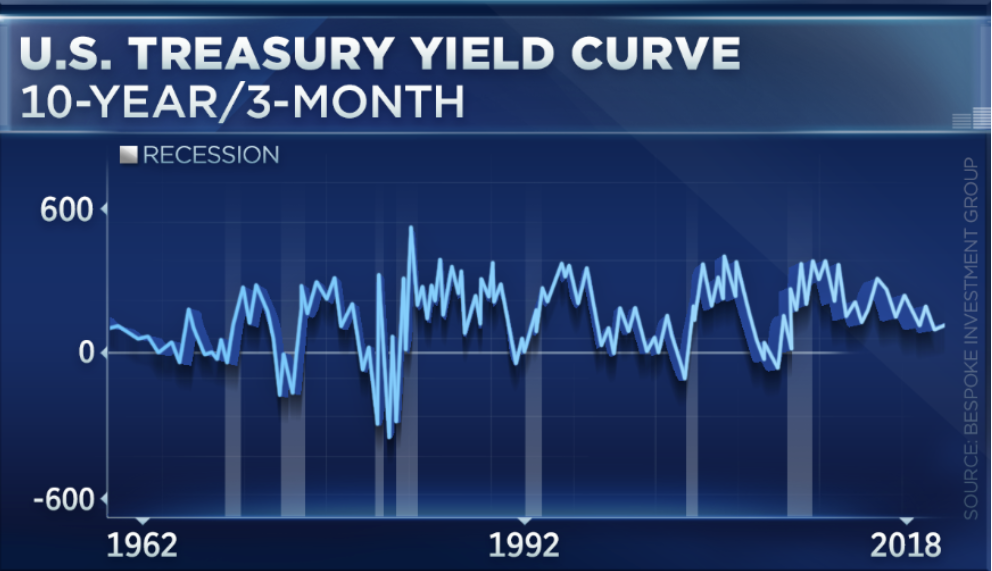
\includegraphics{images/spread_history.png}
    \caption{Spread between 10-year and 3-month bonds. Y-axis is basis points.}
    \label{fig:spread_history}
\end{figure}

